\documentclass[10pt,twocolumn,letterpaper]{article}

\usepackage[dvipsnames,table]{xcolor}
\usepackage{cvpr}
\usepackage{times}
\usepackage{epsfig}
\usepackage{graphicx}
\usepackage{amsmath}
\usepackage{amssymb}
\usepackage{marvosym}
\usepackage{booktabs}

% Include other packages here, before hyperref.
\usepackage{subcaption}
\usepackage{csvsimple}
\usepackage{siunitx}
\usepackage{tabularx}
\usepackage{pgfplots}
\usepackage{tikz}
\usetikzlibrary{
	patterns,
	arrows,
	shapes.misc,
	shapes.symbols,
	calc,
	decorations.text,
	backgrounds,
	decorations.pathreplacing,
	shapes.geometric,
	positioning,
	decorations,
	decorations.markings,
}
\usetikzlibrary{backgrounds}

\makeatletter
\def\pgfmathfloatpow@#1#2{%
    \begingroup%
    \expandafter\pgfmathfloat@decompose@tok#1\relax\pgfmathfloat@a@S\pgfmathfloat@a@Mtok\pgfmathfloat@a@E
    \ifcase\pgfmathfloat@a@S\relax
        % 0 ^ #2 = 0
        \pgfmathfloatcreate{0}{0.0}{0}%
    \else
        \expandafter\pgfmathfloat@decompose@tok#2\relax\pgfmathfloat@a@S\pgfmathfloat@a@Mtok\pgfmathfloat@a@E
        \ifcase\pgfmathfloat@a@S\relax
            % #1 ^ 0 = 1
            \pgfmathfloatcreate{1}{1.0}{0}%
        \or
            % #2 > 0
            \pgfmathfloatpow@@{#1}{#2}%
        \or
            % #2 < 0
            \pgfmathfloatpow@@{#1}{#2}%
        \or
            % #2 = nan
            \edef\pgfmathresult{#2}%
        \or
            % #2 = inf
            \edef\pgfmathresult{#2}%
        \or
            % #2 = -inf
            \pgfmathfloatcreate{0}{0.0}{0}%
        \fi
    \fi
    \pgfmath@smuggleone\pgfmathresult
    \endgroup
}%
\makeatother

\newcolumntype{Y}{>{\centering\arraybackslash}X}
\newcommand{\specialcell}[2][c]{%
  \begin{tabular}[#1]{@{}c@{}}#2\end{tabular}}

\newcommand{\bx}{\mathbf{x}}
\newcommand{\bz}{\mathbf{z}}
\newcommand{\by}{\mathbf{y}}
\newcommand{\br}{\mathbf{r}}
\newcommand{\bp}{\mathbf{p}}

% Method colors
\definecolor{frrn_col}         {RGB}{  0,255,  0}
\definecolor{lrr_col}          {RGB}{255,127,  0}
\definecolor{dilation_col}     {RGB}{255,  0,  0}
\definecolor{enet_col}         {RGB}{220,220,  0}
\definecolor{adelaide_col}     {RGB}{244, 35,232}
\definecolor{segnet_col}       {RGB}{  0,  0,255}
\definecolor{deeplab_col}      {RGB}{  0,255,255}
\definecolor{gray_col}	       {RGB}{180,180,180}

% Lane colors
\definecolor{res_blue}         {RGB}{  0,  0,255}
\definecolor{pool_red}         {RGB}{255,  0,  0}

% Cityscapes colors
\definecolor{csunlabeled}     {RGB}{  0,  0,  0}
\definecolor{csroad}          {RGB}{128, 64,128}
\definecolor{cssidewalk}      {RGB}{244, 35,232}
\definecolor{csbuilding}      {RGB}{ 70, 70, 70}
\definecolor{cswall}          {RGB}{102,102,156}
\definecolor{csfence}         {RGB}{190,153,153}
\definecolor{cspole}          {RGB}{153,153,153}
\definecolor{cstrafficlight}  {RGB}{250,170, 30}
\definecolor{cstrafficsign}   {RGB}{220,220,  0}
\definecolor{csvegetation}    {RGB}{107,142, 35}
\definecolor{csterrain}       {RGB}{152,251,152}
\definecolor{cssky}           {RGB}{ 70,130,180}
\definecolor{csperson}        {RGB}{220, 20, 60}
\definecolor{csrider}         {RGB}{255,  0,  0}
\definecolor{cscar}           {RGB}{  0,  0,142}
\definecolor{cstruck}         {RGB}{  0,  0, 70}
\definecolor{csbus}           {RGB}{  0, 60,100}
\definecolor{cstrain}         {RGB}{  0, 80,100}
\definecolor{csmotorcycle}    {RGB}{  0,  0,230}
\definecolor{csbicycle}       {RGB}{119, 11, 32}

%% -------------------------------------------------------------------------
%% Reduce space between figures and text
%% -------------------------------------------------------------------------
\setlength{\floatsep}{5pt plus2pt minus4pt}
\setlength{\textfloatsep}{5pt plus2pt minus4pt}
\setlength{\dblfloatsep}{5pt plus2pt minus4pt}
\setlength{\dbltextfloatsep}{5pt plus2pt minus4pt}


\newcommand{\imsize}{small_}
%\newcommand{\imsize}{}


%Needed to exclude points from tables
\pgfplotsset{
	discard if not/.style 2 args={
		x filter/.code={
			\edef\tempa{\thisrow{#1}}
			\edef\tempb{#2}
			\ifx\tempa\tempb
			\else
				\def\pgfmathresult{inf}
			\fi
		}
	}
}
\pgfplotsset{
	discard if/.style 2 args={
		x filter/.code={
			\edef\tempa{\thisrow{#1}}
			\edef\tempb{#2}
			\ifx\tempa\tempb
				\def\pgfmathresult{inf}
			\else
			\fi
		}
	}
}
\pgfplotsset{
	discard if not and/.style n args={4}{
		x filter/.code={
		\edef\tempa{\thisrow{#1}}
		\edef\tempb{#2}
		\edef\tempc{\thisrow{#3}}
		\edef\tempd{#4}
		\ifx\tempa\tempb
			\ifx\tempc\tempd
			\else
				\def\pgfmathresult{inf}
			\fi
		\else
			\def\pgfmathresult{inf}
		\fi
		}
	}
}

%for the table
\usepackage{makecell}
\usepackage{ifthen}
\usepackage{stackengine}
\newcommand{\ioucirc}{\begin{Large}
\topinset{\textcolor{black}{$\circ$}}{\textcolor{black}{$\circ$}}{2.5pt}{}
\end{Large}}
\newcommand{\mycirc}[1][black]{\begin{tikzpicture}[baseline=-0.75ex]
\draw [fill=#1, #1] (0,0) circle (2.5pt);
\draw[transparent] (0,0) -- (-7pt, 0);
\draw[transparent] (0,0) -- (4.8pt, 0);
\end{tikzpicture} }


% If you comment hyperref and then uncomment it, you should delete
% egpaper.aux before re-running latex.  (Or just hit 'q' on the first latex
% run, let it finish, and you should be clear).
\usepackage[pagebackref=true,breaklinks=true,letterpaper=true,colorlinks,bookmarks=false]{hyperref}

%\cvprfinalcopy % *** Uncomment this line for the final submission

\def\cvprPaperID{1691} % *** Enter the CVPR Paper ID here
\def\httilde{\mbox{\tt\raisebox{-.5ex}{\symbol{126}}}}
\newcommand{\TODO}[1]{\textcolor{red}{#1}}
\newcommand{\DOWE}[1]{\textcolor{green}{#1}}
\newcommand{\PAR}[1]{\vskip4pt \noindent {\bf #1~}}
\newcommand{\PARbegin}[1]{\noindent {\bf #1~}}
% Pages are numbered in submission mode, and unnumbered in camera-ready
\ifcvprfinal\pagestyle{empty}\fi
\begin{document}

%%%%%%%%% TITLE
\title{Full-Resolution Residual Networks for Semantic Segmentation in Street Scenes}

\author{Tobias Pohlen \hspace{10mm} Alexander Hermans \hspace{10mm} Markus Mathias \hspace{10mm} Bastian Leibe\\
Visual Computing Institute\\
RWTH Aachen University\\
{\tt\small \{pohlen, hermans, leibe\}@vision.rwth-aachen.de}
% For a paper whose authors are all at the same institution,
% omit the following lines up until the closing ``}''.
% Additional authors and addresses can be added with ``\and'',
% just like the second author.
% To save space, use either the email address or home page, not both
}

\maketitle
%\thispagestyle{empty}

\definecolor{nn-input-color}{RGB}{187,187,187}
\definecolor{nn-fc-color}{RGB}{251,255,123}
\definecolor{nn-conv-color}{RGB}{208,225,166}
\definecolor{nn-bias-color}{RGB}{225,222,166}
\definecolor{nn-bn-color}{RGB}{243,140,136}
\definecolor{nn-relu-color}{RGB}{232,151,218}
\definecolor{nn-softmax-color}{RGB}{251,255,2}
\definecolor{nn-pool-color}{RGB}{238,189,154}
\definecolor{nn-unpool-color}{RGB}{154,189,238}
\definecolor{nn-concat-color}{RGB}{191,132,253}
\definecolor{nn-sum-color}{RGB}{127,255,255}
\definecolor{nn-cu-color}{RGB}{255,216,0}

\tikzstyle{nn-node}=[draw, thick, rounded corners=5pt]
\tikzstyle{nn-teaser}=[minimum height=0.6cm, minimum width=0.6cm]
\tikzstyle{nn-minor}=[minimum height=0.45cm, minimum width=0.45cm, Gray!70, text=Black]
\tikzstyle{nn-edge}=[thick, rounded corners=3pt]
\tikzstyle{nn-arrow}=[->, >=stealth]

\tikzstyle{nn-input}=[fill=nn-input-color]
\tikzstyle{nn-fc}=[fill=nn-fc-color]
\tikzstyle{nn-conv}=[fill=nn-conv-color]
\tikzstyle{nn-bias}=[fill=nn-bias-color]
\tikzstyle{nn-bn}=[fill=nn-bn-color]
\tikzstyle{nn-relu}=[fill=nn-relu-color]
\tikzstyle{nn-softmax}=[fill=nn-softmax-color]
\tikzstyle{nn-pool}=[fill=nn-pool-color]
\tikzstyle{nn-unpool}=[fill=nn-unpool-color]
\tikzstyle{nn-concat}=[fill=nn-concat-color]
\tikzstyle{nn-sum}=[fill=nn-sum-color]
\tikzstyle{nn-cu}=[fill=nn-cu-color]
%%%%%%%%% ABSTRACT
%\begin{abstract}
%In this supplementary material 
%We provide additional details to our gamma augmentation, detailed training curves for our baseline experiment and additional qualitative results.
%Furthermore, we provide our output for the Cityscapes demo video for a better qualitative understanding of our method.
%\end{abstract}


\section{Gamma Augmentation}
Gamma augmentation is an augmentation method that varies the image contrast and brightness.
Assume the intensity values of an image are scaled to the unit interval $[0, 1]$.
Then gamma augmentation applies the intensity transformation $x \mapsto x^\gamma$ for a randomly sampled augmentation parameter $\gamma > 0$. 
However, sampling the augmentation parameter $\gamma$ is not trivial.
Naively drawing samples from a uniform or truncated Gaussian distribution with a mean of $1$ results in a noticeable bias (Figure \ref{fig:gamma_a}).
In order to reduce the bias, we deduce a novel sampling schema for $\gamma$. 

Let $U$ be a random variable that is implicitly defined as the solution to the fixed-point problem
\begin{align}
  \label{eq:61}
  1 - U^\gamma = U.
\end{align}
Our goal is to find $\gamma$ such that $\mathbb{E}_U[U] = 0.5$. 
The key idea to solving this problem is to look at the deviation of $U$ from $0.5$. 
Let $Z$ be this deviation. Then (\ref{eq:61}) is equivalent to 
\begin{align}
  \label{eq:62}
  \left(0.5 - \frac{1}{\sqrt{2}}Z \right)^\gamma = 0.5 + \frac{1}{\sqrt{2}}Z.
\end{align}
Now $\mathbb{E}_U[U] = 0.5$ implies $\mathbb{E}_Z[Z] = 0$ and solving (\ref{eq:62}) for $\gamma$ yields
\begin{align}
  \label{eq:63}
  \gamma = \frac{\log\left(0.5 + 2^{-0.5} Z\right)}{\log \left(0.5 - 2^{-0.5} Z\right)}.
\end{align}
Hence, without solving for the implicitly defined variable $U$ explicitly, we found a transformation of a zero-mean random variable $Z$ such that $\gamma$ has the desired properties. 
Because $Z$ was defined to be the offset from $0.5$ and $U \in [0, 1]$, it follows $Z \in [-0.5, 0.5]$.
We are free to choose any distribution such that $Z$ has zero mean and falls into the range $[-0.5, 0.5]$. 
For simplicity reasons, we choose $Z$ to be uniformly distributed over $[-a, a]$ where $a \in [0, 0.5]$ determines the strength of the augmentation. 
Figure \ref{fig:gamma_b} illustrates the obvious bias reduction.

			\newcommand{\samplevar}{50}
			\begin{figure}[t]
				\begin{subfigure}{0.48\linewidth}
				\centering
					\resizebox{\linewidth}{!}{
					\begin{tikzpicture}[tight background]
						\begin{axis}[xmin=0, xmax=1, ymin=0, ymax=1, enlargelimits=false,
								grid=both,
								major grid style={line width=.1pt, draw=gray!40},
								ylabel style={font=\footnotesize},
								xlabel style={font=\footnotesize},
								xtick pos=left,
								ytick pos=left,
								every tick label/.append style={font=\footnotesize}, ]
						\addplot[blue, ultra thin, opacity=0.6, domain=0:1, samples=\samplevar] {pow(x, 1.128500)};
						\addplot[blue, ultra thin, opacity=0.6, domain=0:1, samples=\samplevar] {pow(x, 1.595996)};
						\addplot[blue, ultra thin, opacity=0.6, domain=0:1, samples=\samplevar] {pow(x, 0.515135)};
						\addplot[blue, ultra thin, opacity=0.6, domain=0:1, samples=\samplevar] {pow(x, 0.565716)};
						\addplot[blue, ultra thin, opacity=0.6, domain=0:1, samples=\samplevar] {pow(x, 1.102926)};
						\addplot[blue, ultra thin, opacity=0.6, domain=0:1, samples=\samplevar] {pow(x, 0.925790)};
						\addplot[blue, ultra thin, opacity=0.6, domain=0:1, samples=\samplevar] {pow(x, 0.939443)};
						\addplot[blue, ultra thin, opacity=0.6, domain=0:1, samples=\samplevar] {pow(x, 1.054726)};
						\addplot[blue, ultra thin, opacity=0.6, domain=0:1, samples=\samplevar] {pow(x, 0.255801)};
						\addplot[blue, ultra thin, opacity=0.6, domain=0:1, samples=\samplevar] {pow(x, 0.738766)};
						\addplot[blue, ultra thin, opacity=0.6, domain=0:1, samples=\samplevar] {pow(x, 1.448811)};
						\addplot[blue, ultra thin, opacity=0.6, domain=0:1, samples=\samplevar] {pow(x, 1.297795)};
						\addplot[blue, ultra thin, opacity=0.6, domain=0:1, samples=\samplevar] {pow(x, 0.477621)};
						\addplot[blue, ultra thin, opacity=0.6, domain=0:1, samples=\samplevar] {pow(x, 0.948280)};
						\addplot[blue, ultra thin, opacity=0.6, domain=0:1, samples=\samplevar] {pow(x, 0.356212)};
						\addplot[blue, ultra thin, opacity=0.6, domain=0:1, samples=\samplevar] {pow(x, 0.465451)};
						\addplot[blue, ultra thin, opacity=0.6, domain=0:1, samples=\samplevar] {pow(x, 0.537862)};
						\addplot[blue, ultra thin, opacity=0.6, domain=0:1, samples=\samplevar] {pow(x, 1.737717)};
						\addplot[blue, ultra thin, opacity=0.6, domain=0:1, samples=\samplevar] {pow(x, 1.521992)};
						\addplot[blue, ultra thin, opacity=0.6, domain=0:1, samples=\samplevar] {pow(x, 0.855151)};
						\addplot[blue, ultra thin, opacity=0.6, domain=0:1, samples=\samplevar] {pow(x, 0.815888)};
						\addplot[blue, ultra thin, opacity=0.6, domain=0:1, samples=\samplevar] {pow(x, 1.044113)};
						\addplot[blue, ultra thin, opacity=0.6, domain=0:1, samples=\samplevar] {pow(x, 0.577801)};
						\addplot[blue, ultra thin, opacity=0.6, domain=0:1, samples=\samplevar] {pow(x, 0.467020)};
						\addplot[blue, ultra thin, opacity=0.6, domain=0:1, samples=\samplevar] {pow(x, 0.656226)};
						\addplot[blue, ultra thin, opacity=0.6, domain=0:1, samples=\samplevar] {pow(x, 0.740813)};
						\addplot[blue, ultra thin, opacity=0.6, domain=0:1, samples=\samplevar] {pow(x, 0.653977)};
						\addplot[blue, ultra thin, opacity=0.6, domain=0:1, samples=\samplevar] {pow(x, 1.394314)};
						\addplot[blue, ultra thin, opacity=0.6, domain=0:1, samples=\samplevar] {pow(x, 0.470037)};
						\addplot[blue, ultra thin, opacity=0.6, domain=0:1, samples=\samplevar] {pow(x, 1.386796)};
						\addplot[blue, ultra thin, opacity=0.6, domain=0:1, samples=\samplevar] {pow(x, 0.408322)};
						\addplot[blue, ultra thin, opacity=0.6, domain=0:1, samples=\samplevar] {pow(x, 1.082375)};
						\addplot[blue, ultra thin, opacity=0.6, domain=0:1, samples=\samplevar] {pow(x, 1.033171)};
						\addplot[blue, ultra thin, opacity=0.6, domain=0:1, samples=\samplevar] {pow(x, 0.320815)};
						\addplot[blue, ultra thin, opacity=0.6, domain=0:1, samples=\samplevar] {pow(x, 1.202513)};
						\addplot[blue, ultra thin, opacity=0.6, domain=0:1, samples=\samplevar] {pow(x, 1.249883)};
						\addplot[blue, ultra thin, opacity=0.6, domain=0:1, samples=\samplevar] {pow(x, 1.169531)};
						\addplot[blue, ultra thin, opacity=0.6, domain=0:1, samples=\samplevar] {pow(x, 1.586669)};
						\addplot[blue, ultra thin, opacity=0.6, domain=0:1, samples=\samplevar] {pow(x, 0.292345)};
						\addplot[blue, ultra thin, opacity=0.6, domain=0:1, samples=\samplevar] {pow(x, 0.518001)};
						\addplot[blue, ultra thin, opacity=0.6, domain=0:1, samples=\samplevar] {pow(x, 1.343989)};
						\addplot[blue, ultra thin, opacity=0.6, domain=0:1, samples=\samplevar] {pow(x, 0.689026)};
						\addplot[blue, ultra thin, opacity=0.6, domain=0:1, samples=\samplevar] {pow(x, 0.925999)};
						\addplot[blue, ultra thin, opacity=0.6, domain=0:1, samples=\samplevar] {pow(x, 1.539841)};
						\addplot[blue, ultra thin, opacity=0.6, domain=0:1, samples=\samplevar] {pow(x, 1.630720)};
						\addplot[blue, ultra thin, opacity=0.6, domain=0:1, samples=\samplevar] {pow(x, 1.343801)};
						\addplot[blue, ultra thin, opacity=0.6, domain=0:1, samples=\samplevar] {pow(x, 1.724412)};
						\addplot[blue, ultra thin, opacity=0.6, domain=0:1, samples=\samplevar] {pow(x, 1.337520)};
						\addplot[blue, ultra thin, opacity=0.6, domain=0:1, samples=\samplevar] {pow(x, 1.225040)};
						\addplot[blue, ultra thin, opacity=0.6, domain=0:1, samples=\samplevar] {pow(x, 1.358421)};
						\end{axis}
					\end{tikzpicture}}
					\caption{}
					\label{fig:gamma_a}
				\end{subfigure}%
				\begin{subfigure}{0.48\linewidth}
				\centering
					\resizebox{\linewidth}{!}{
					\begin{tikzpicture}[tight background]
						\begin{axis}[xmin=0, xmax=1, ymin=0, ymax=1, enlargelimits=false,
								grid=both,
								major grid style={line width=.1pt, draw=gray!40},
								ylabel style={font=\footnotesize},
								xlabel style={font=\footnotesize},
								xtick pos=left,
								ytick pos=left,
								every tick label/.append style={font=\footnotesize}, ]
						\addplot[blue, ultra thin, opacity=0.6, domain=0:1, samples=\samplevar] {pow(x, 0.234318)};
						\addplot[blue, ultra thin, opacity=0.6, domain=0:1, samples=\samplevar] {pow(x, 0.412055)};
						\addplot[blue, ultra thin, opacity=0.6, domain=0:1, samples=\samplevar] {pow(x, 3.340263)};
						\addplot[blue, ultra thin, opacity=0.6, domain=0:1, samples=\samplevar] {pow(x, 1.632278)};
						\addplot[blue, ultra thin, opacity=0.6, domain=0:1, samples=\samplevar] {pow(x, 2.717150)};
						\addplot[blue, ultra thin, opacity=0.6, domain=0:1, samples=\samplevar] {pow(x, 1.499970)};
						\addplot[blue, ultra thin, opacity=0.6, domain=0:1, samples=\samplevar] {pow(x, 1.280350)};
						\addplot[blue, ultra thin, opacity=0.6, domain=0:1, samples=\samplevar] {pow(x, 1.064177)};
						\addplot[blue, ultra thin, opacity=0.6, domain=0:1, samples=\samplevar] {pow(x, 0.555242)};
						\addplot[blue, ultra thin, opacity=0.6, domain=0:1, samples=\samplevar] {pow(x, 1.161980)};
						\addplot[blue, ultra thin, opacity=0.6, domain=0:1, samples=\samplevar] {pow(x, 1.437325)};
						\addplot[blue, ultra thin, opacity=0.6, domain=0:1, samples=\samplevar] {pow(x, 0.551097)};
						\addplot[blue, ultra thin, opacity=0.6, domain=0:1, samples=\samplevar] {pow(x, 1.207614)};
						\addplot[blue, ultra thin, opacity=0.6, domain=0:1, samples=\samplevar] {pow(x, 2.741176)};
						\addplot[blue, ultra thin, opacity=0.6, domain=0:1, samples=\samplevar] {pow(x, 1.668427)};
						\addplot[blue, ultra thin, opacity=0.6, domain=0:1, samples=\samplevar] {pow(x, 0.302076)};
						\addplot[blue, ultra thin, opacity=0.6, domain=0:1, samples=\samplevar] {pow(x, 2.107278)};
						\addplot[blue, ultra thin, opacity=0.6, domain=0:1, samples=\samplevar] {pow(x, 1.177167)};
						\addplot[blue, ultra thin, opacity=0.6, domain=0:1, samples=\samplevar] {pow(x, 0.637523)};
						\addplot[blue, ultra thin, opacity=0.6, domain=0:1, samples=\samplevar] {pow(x, 0.375384)};
						\addplot[blue, ultra thin, opacity=0.6, domain=0:1, samples=\samplevar] {pow(x, 0.855881)};
						\addplot[blue, ultra thin, opacity=0.6, domain=0:1, samples=\samplevar] {pow(x, 3.791002)};
						\addplot[blue, ultra thin, opacity=0.6, domain=0:1, samples=\samplevar] {pow(x, 2.848499)};
						\addplot[blue, ultra thin, opacity=0.6, domain=0:1, samples=\samplevar] {pow(x, 0.384804)};
						\addplot[blue, ultra thin, opacity=0.6, domain=0:1, samples=\samplevar] {pow(x, 0.275975)};
						\addplot[blue, ultra thin, opacity=0.6, domain=0:1, samples=\samplevar] {pow(x, 0.607875)};
						\addplot[blue, ultra thin, opacity=0.6, domain=0:1, samples=\samplevar] {pow(x, 0.265034)};
						\addplot[blue, ultra thin, opacity=0.6, domain=0:1, samples=\samplevar] {pow(x, 0.638853)};
						\addplot[blue, ultra thin, opacity=0.6, domain=0:1, samples=\samplevar] {pow(x, 3.452812)};
						\addplot[blue, ultra thin, opacity=0.6, domain=0:1, samples=\samplevar] {pow(x, 0.319410)};
						\addplot[blue, ultra thin, opacity=0.6, domain=0:1, samples=\samplevar] {pow(x, 1.076541)};
						\addplot[blue, ultra thin, opacity=0.6, domain=0:1, samples=\samplevar] {pow(x, 0.295365)};
						\addplot[blue, ultra thin, opacity=0.6, domain=0:1, samples=\samplevar] {pow(x, 0.654122)};
						\addplot[blue, ultra thin, opacity=0.6, domain=0:1, samples=\samplevar] {pow(x, 3.693893)};
						\addplot[blue, ultra thin, opacity=0.6, domain=0:1, samples=\samplevar] {pow(x, 0.227724)};
						\addplot[blue, ultra thin, opacity=0.6, domain=0:1, samples=\samplevar] {pow(x, 1.388102)};
						\addplot[blue, ultra thin, opacity=0.6, domain=0:1, samples=\samplevar] {pow(x, 2.709128)};
						\addplot[blue, ultra thin, opacity=0.6, domain=0:1, samples=\samplevar] {pow(x, 1.664260)};
						\addplot[blue, ultra thin, opacity=0.6, domain=0:1, samples=\samplevar] {pow(x, 0.327375)};
						\addplot[blue, ultra thin, opacity=0.6, domain=0:1, samples=\samplevar] {pow(x, 0.454886)};
						\addplot[blue, ultra thin, opacity=0.6, domain=0:1, samples=\samplevar] {pow(x, 0.227395)};
						\addplot[blue, ultra thin, opacity=0.6, domain=0:1, samples=\samplevar] {pow(x, 1.013165)};
						\addplot[blue, ultra thin, opacity=0.6, domain=0:1, samples=\samplevar] {pow(x, 1.461112)};
						\addplot[blue, ultra thin, opacity=0.6, domain=0:1, samples=\samplevar] {pow(x, 0.936760)};
						\addplot[blue, ultra thin, opacity=0.6, domain=0:1, samples=\samplevar] {pow(x, 0.237725)};
						\addplot[blue, ultra thin, opacity=0.6, domain=0:1, samples=\samplevar] {pow(x, 2.636775)};
						\addplot[blue, ultra thin, opacity=0.6, domain=0:1, samples=\samplevar] {pow(x, 4.002555)};
						\addplot[blue, ultra thin, opacity=0.6, domain=0:1, samples=\samplevar] {pow(x, 1.869112)};
						\addplot[blue, ultra thin, opacity=0.6, domain=0:1, samples=\samplevar] {pow(x, 0.711069)};
						\addplot[blue, ultra thin, opacity=0.6, domain=0:1, samples=\samplevar] {pow(x, 0.541572)};
						\end{axis}
					\end{tikzpicture}}
					\caption{}
					\label{fig:gamma_b}
				\end{subfigure}%
				\caption{
					Both plots show the function $x \mapsto x^\gamma$ for 50 samples of $\gamma$.
					In plot (a), $\gamma$ is sampled uniformly at random from the interval $[0.25, 1.75]$.
					%In plot (b), we apply the nonlinear transformation $\gamma = \frac{\log(0.5 + 2^{-0.5} Z)}{\log(0.5 - 2^{-0.5} Z)}$ where $Z$ is sampled uniformly at random from the interval $[-a, a]$ for $a = 0.35$, which reduces the bias.
					In plot (b), we use Equation \ref{eq:63} where $Z$ is sampled uniformly from the interval $[-0.35, 0.35]$.
					Our new sampling reduces the bias.
					}
				\label{fig:gamma}
			\end{figure}

%%%%%%%%% BODY TEXT
\section{Baseline Evaluation}
In Section 5.2 of the main paper, we describe the setting of our baseline method (Residual Network Baseline) and compare it to our FRRN A network. 
To emphasize on a proper training procedure of both baselines, Figure \ref{fig:baseline} shows the mean IoU score on the validation set over time. 
We can see that our model outperforms the baseline with a significant margin and both methods are trained until convergence.

\pgfplotstableread[col sep=tab]{baseline.csv}\baselinedata
\begin{figure}[h]
	\resizebox{\linewidth}{!}{
	\begin{tikzpicture}[tight background]
		\begin{axis}[
   width=\linewidth,
   xlabel=Iteration,
   ylabel=IoU score,
	       	grid=both, 
	       	major grid style={line width=.1pt, draw=gray!40}, 
	       	legend style={font=\tiny, at={(0.95, 0.05)},anchor=south east},
	       	legend columns=1,
	       	ylabel style={font=\footnotesize}, 
	       	xlabel style={font=\footnotesize}, 
	       	height=6cm, 
	       	xtick pos=left, 
	       	ytick pos=left, 
	       	xtick style={draw=none},  
	       	every tick label/.append style={font=\footnotesize}, 
	       	xmin=0, 
	       	ymin=0, 
	       	ymax=80, 
	       	xmax=45000,
	       	scaled ticks=false, 
	       	tick label style={/pgf/number format/fixed}
	       	]
	       	
			\addplot[blue, dashed, no marks, y filter/.code={\pgfmathparse{\pgfmathresult*100}\pgfmathresult}] table[x index=0, y index=1] \baselinedata;
			\addplot[red, dashed, no marks, y filter/.code={\pgfmathparse{\pgfmathresult*100}\pgfmathresult}] table[x index=0, y index=2] \baselinedata;
			\addplot[blue, no marks, y filter/.code={\pgfmathparse{\pgfmathresult*100}\pgfmathresult}] table[x index=0, y index=3] \baselinedata;
			\addplot[red, no marks, y filter/.code={\pgfmathparse{\pgfmathresult*100}\pgfmathresult}] table[x index=0, y index=4] \baselinedata;
			
			\legend{FRRN A, ResNet with long-range skips, current best FRRN A, current best ResNet}
		\end{axis}
	\end{tikzpicture}} 
	\caption{
		The plot shows the IoU score on the Cityscapes validation set as a function of the number of training iterations for the baseline architecture and FRRN A.
		The solid lines show the best IoU score up to iteration $N$.
	}
	\label{fig:baseline}
\end{figure}


\newcommand{\resimlinetwo}[1]{\includegraphics[width=1\linewidth]{images/results/ims/\imsize#1}&
          \includegraphics[width=1\linewidth]{images/results/gt/\imsize#1}&
          \includegraphics[width=1\linewidth]{images/results/ours/\imsize#1}&
          \includegraphics[width=1\linewidth]{images/results/lrr/\imsize#1}\\[-2pt]}

\begin{figure*}[t]
    \setlength\tabcolsep{1pt}
    \begin{tabularx}{\linewidth}{@{}YYYYYY@{}}
      Image & Ground Truth & Ours & LRR \cite{Ghiasi16ECCV}\\
      %\resimlinetwo{frankfurt_000000_007365}
      %\resimlinetwo{frankfurt_000000_010351}
      \resimlinetwo{frankfurt_000001_077233}
      \resimlinetwo{lindau_000018_000019}
      %\resimlinetwo{lindau_000024_000019}
      \resimlinetwo{munster_000065_000019}
      %\resimlinetwo{munster_000055_000019}
      %\resimlinetwo{munster_000129_000019}
      \resimlinetwo{munster_000097_000019}
      \resimlinetwo{munster_000128_000019}
      \resimlinetwo{munster_000157_000019}
      \resimlinetwo{munster_000167_000019}
      \resimlinetwo{frankfurt_000001_058914}
    \end{tabularx}
    \resizebox{\linewidth}{!}{
      \begin{tikzpicture}[tight background, scale=0.75, every node/.style={font=\large}]
	\draw[white, fill=csunlabeled, draw=white] (0,0) rectangle (1 * 4, 1) node[pos=0.5] {Void};
	\draw[white, fill=csroad, draw=white] (1 * 4,0) rectangle (2 * 4, 1) node[pos=0.5] {Road};
	\draw[white, fill=cssidewalk, draw=white] (2 * 4,0) rectangle (3 * 4, 1) node[pos=0.5] {Sidewalk};
	\draw[white, fill=csbuilding, draw=white] (3 * 4,0) rectangle (4 * 4, 1) node[pos=0.5] {Building};
	\draw[white, fill=cswall, draw=white] (4 * 4,-0) rectangle (5 * 4, 1) node[pos=0.5] {Wall};
	\draw[black, fill=csfence, draw=white] (5 * 4,-0) rectangle (6 * 4, 1) node[pos=0.5] {Fence};
	\draw[white, fill=cspole, draw=white] (6 * 4,-0) rectangle (7 * 4, 1) node[pos=0.5] {Pole};
	\draw[white, fill=cstrafficlight, draw=white] (7 * 4,-0) rectangle (8 * 4, 1) node[pos=0.5] {Traffic Light};
	\draw[black, fill=cstrafficsign, draw=white] (8 * 4,-0) rectangle (9 * 4, 1) node[pos=0.5] {Traffic Sign};
	\draw[white, fill=csvegetation, draw=white] (9 * 4,-0) rectangle (10 * 4, 1) node[pos=0.5] {Vegetation};

	\draw[black, fill=csterrain, draw=white] (0 * 4,-1) rectangle (1 * 4, 0) node[pos=0.5] {Terrain};
	\draw[white, fill=cssky, draw=white] (1 * 4,-1) rectangle (4 * 2, 0) node[pos=0.5] {Sky};
	\draw[white, fill=csperson, draw=white] (2 * 4,-1) rectangle (3 * 4, 0) node[pos=0.5] {Person};
	\draw[white, fill=csrider, draw=white] (3 * 4,-1) rectangle (4 * 4, 0) node[pos=0.5] {Rider};
	\draw[white, fill=cscar, draw=white] (4 * 4,-1) rectangle (5 * 4, 0) node[pos=0.5] {Car};
	\draw[white, fill=cstruck, draw=white] (5 * 4,-1) rectangle (6 * 4, 0) node[pos=0.5] {Truck};
	\draw[white, fill=csbus, draw=white] (6 * 4,-1) rectangle (7 * 4, 0) node[pos=0.5] {Bus};
	\draw[white, fill=cstrain, draw=white] (7 * 4,-1) rectangle (8 * 4, 0) node[pos=0.5] {Train};
	\draw[white, fill=csmotorcycle, draw=white] (8 * 4,-1) rectangle (9 * 4, 0) node[pos=0.5] {Motorcycle};
	\draw[white, fill=csbicycle, draw=white] (9 * 4,-1) rectangle (10 * 4, 0) node[pos=0.5] {Bicycle};
\end{tikzpicture}
    }
    \caption{
      Additional qualitative results on the Cityscapes validation set.
      We omit the comparison to Dilation \cite{Yu16ICLR} in order to show bigger images here.
    }
    \label{fig:qualitative_appendix}
\end{figure*}

\section{Qualitative Results}
\vspace*{-6pt}
Figure \ref{fig:qualitative_appendix} shows and compares addtional output labelings of our method.
Please also consult our labeled video sequence to gain a better sense of the quality of our method.
\textcolor{white}{We all know Latex is a pain.}
%The segmentation masks of the individual frames are predicted independently from another.
%Hence, there is no temporal component.
%However, in contrast to the qualitative results shown in Figure \ref{fig:qualitative_appendix}, we performed noise injection at runtime in order to obtain the segmentation.
%To this end, we obtain multiple versions of each frame by applying the augmentation steps described before and then average the predictions over all versions.
%This results in an improved visual temporal consistency of the segmentation masks.
%The video can also be seen here: youtubeLINK


{\small
\bibliographystyle{ieee}
\bibliography{abbrev_short,egbib}
}

\end{document}
